% Created 2021-01-15 ven. 08:02
% Intended LaTeX compiler: pdflatex
\documentclass[presentation]{beamer}
\usepackage[utf8]{inputenc}
\usepackage[T1]{fontenc}
\usepackage{graphicx}
\usepackage{grffile}
\usepackage{longtable}
\usepackage{wrapfig}
\usepackage{rotating}
\usepackage[normalem]{ulem}
\usepackage{amsmath}
\usepackage{textcomp}
\usepackage{amssymb}
\usepackage{capt-of}
\usepackage{hyperref}
\usepackage{color}
\usetheme{CambridgeUS}
\setbeamertemplate{navigation symbols}{} % pas de barre de navigation
\usepackage[english]{babel}
\usepackage{lmodern}
\usepackage[matha,mathb]{mathabx}
\usepackage{subfig}
\usepackage{mdframed}
\usepackage{minted}
\usemintedstyle{friendly} % set style if needed, see https://frama.link/jfRr8Lpj
\mdfdefinestyle{mystyle}{linecolor=gray!30,backgroundcolor=gray!30}
\BeforeBeginEnvironment{minted}{%
\small \begin{mdframed}[style=mystyle]}
\AfterEndEnvironment{minted}{%
\end{mdframed} \medskip \normalsize}
\usepackage{float}
\usepackage{url}
%% Formatting of verbatim outputs (i.e., outputs of R results):
\DefineVerbatimEnvironment{verbatim}{Verbatim}{%
fontsize = \small,
frame = leftline,
formatcom = {\color{gray!97}}
}
\setbeamertemplate{caption}[numbered]
%% Perso colors
\definecolor{PalePurple}{RGB}{127, 90, 182}
\definecolor{DarkPurple}{RGB}{98, 36, 134}
\definecolor{grey}{RGB}{51, 63, 72}
\setbeamercolor{title}{fg=white, bg=DarkPurple}
\setbeamercolor{frametitle}{fg=black}
\setbeamercolor{structure}{fg=PalePurple}
\setbeamercolor{section in head/foot}{fg=white, bg=PalePurple}
\setbeamercolor{subsection in head/foot}{fg=DarkPurple}
\setbeamercolor{title in head/foot}{fg=white, bg=DarkPurple}
\setbeamercolor{date in head/foot}{fg=grey}
\setbeamercolor{block title}{fg=white, bg=DarkPurple}
\setbeamercolor{block body}{bg=gray!20}
%% Structure of a slide :
\setbeamertemplate{footline}
{
\leavevmode%
\hbox{%
\begin{beamercolorbox}[wd=.75\paperwidth,ht=2.25ex,dp=1ex,center]{title in head/foot}%
\usebeamerfont{author in head/foot}\inserttitle
\end{beamercolorbox}%
%\begin{beamercolorbox}[wd=.3\paperwidth,ht=2.25ex,dp=1ex,center]{section in head/foot}%
%\usebeamerfont{title in head/foot}\insertsection
%\end{beamercolorbox}%
\begin{beamercolorbox}[wd=.25\paperwidth,ht=2.25ex,dp=1ex,center]{date in head/foot}%
\insertframenumber{} / \inserttotalframenumber\hspace*{1ex}
\end{beamercolorbox}}%
\vskip0pt%
}
\DeclareUnicodeCharacter{2514}{\mbox{\kern.23em \vrule height2.2exdepth-1.8ptwidth.4pt\vrule height2.2ptdepth-1.8ptwidth.23em}}
\DeclareUnicodeCharacter{2500}{\mbox{\vrule height2.2ptdepth-1.8ptwidth.5em}}
\setlength{\parskip}{5pt}
\usetheme{default}
\author{Frédéric Santos\thanks{frederic.santos@u-bordeaux.fr}}
\date{\today}
\title{Customizing and extending Emacs Speaks Statistics}
\hypersetup{
 pdfauthor={Frédéric Santos},
 pdftitle={Customizing and extending Emacs Speaks Statistics},
 pdfkeywords={},
 pdfsubject={},
 pdfcreator={Emacs 27.1 (Org mode 9.4.4)}, 
 pdflang={English}}
\begin{document}

\maketitle


\section{Introductory words}
\label{sec:org118db03}
\subsection{Filling your Emacs init file}
\label{sec:org06180f8}
\begin{frame}[label={sec:org1d01855},fragile]{A word about \texttt{use-package}}
 In this document, several pieces of Emacs Lisp code will be proposed so that you can use them in your init file.

It is assumed that you use \href{https://jwiegley.github.io/use-package/}{\texttt{use-package}} for your init file: the Emacs Lisp code can be adapted in a straightforward manner if you do not use it.

As a reminder, this is the minimal code to add in your init file so as to use \texttt{use-package}, once it has been installed:

\begin{minted}[]{common-lisp}
;; Make sure that use-package is installed:
(unless (package-installed-p 'use-package)
  (package-refresh-contents)
  (package-install 'use-package))
;; Load use-package:
(eval-when-compile
  (require 'use-package))
\end{minted}
\end{frame}

\section{ESS customization}
\label{sec:orgdf7a0a3}
\subsection{Visibility of evaluation}
\label{sec:orgca1c513}
\subsection{Window management}
\label{sec:org6e9173d}
\subsection{Syntax highlighting}
\label{sec:org0b717be}
\subsection{Syntax checker}
\label{sec:org1c9f1c3}
\subsection{Rdired buffers}
\label{sec:orga50892e}

\section{Some useful Emacs packages}
\label{sec:org3b5d14c}
\subsection{company}
\label{sec:org8825e59}
\subsection{company-quickhelp}
\label{sec:org2f600f5}
\begin{frame}[fragile,allowframebreaks,label=]{Documentation popups}
 \href{https://github.com/company-mode/company-quickhelp}{\texttt{company-quickhelp}} allows for documentation popups, e.g. to further describe function arguments.

\begin{figure}[htbp]
\centering
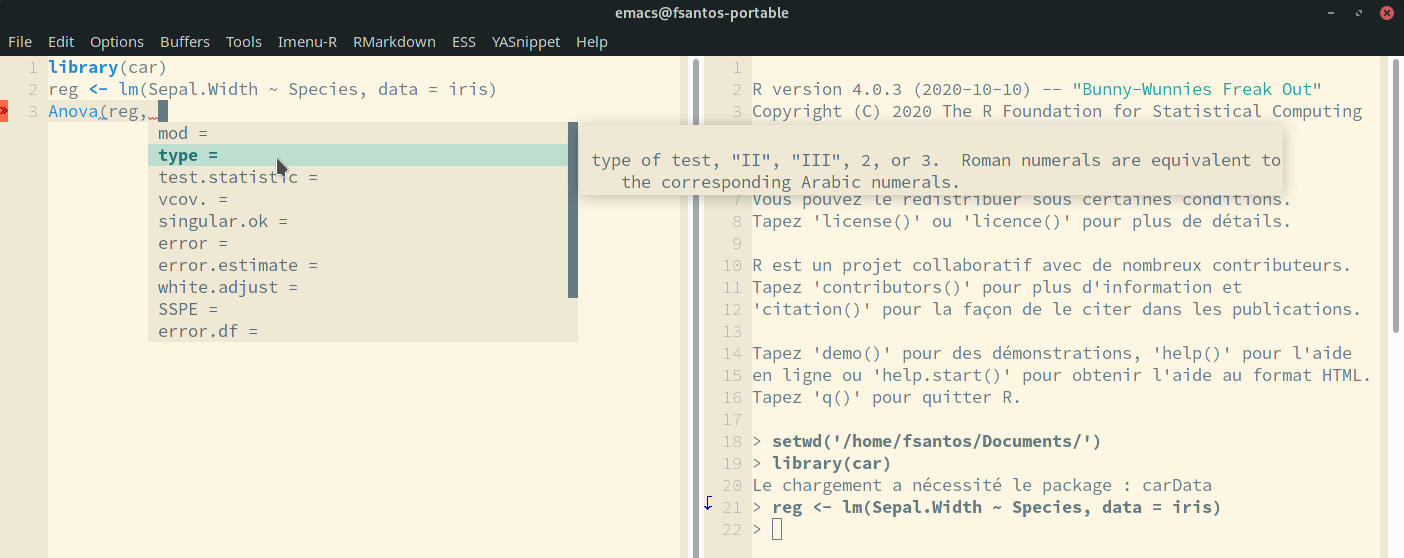
\includegraphics[width=\textwidth]{./images/company-quickhelp.png}
\caption{Documentation popups with \texttt{company-quickhelp}.}
\end{figure}

The minimal elisp code to add to your init file is straightforward:

\begin{minted}[]{common-lisp}
(use-package company-quickhelp
  :ensure t
  :config
  ;; Load company-quickhelp globally:
  (company-quickhelp-mode)
  ;; Time before display of documentation popup:
  (setq company-quickhelp-delay 0.3))
\end{minted}

By default, the documentation popup is shown automatically. You can adjust the time before the popup shows up by customizing the variable \texttt{company-quickhelp-delay}.
\end{frame}

\subsection{yasnippet}
\label{sec:org49d0515}
\begin{frame}[label={sec:orge714f83},fragile]{Code snippets}
 \href{https://github.com/joaotavora/yasnippet}{\texttt{yasnippet}} is an Emacs package allowing for the expansion of whole pieces of code you often use (\emph{snippets}) from one given abbreviation. 

\begin{block}{Key features of \texttt{yasnippet}}
\begin{itemize}
\item All code snippets are stored as plain-text files in one given directory, so that they are easy to share with other people, and can be easily version controlled.
\item As a corollary, it is also easy to retrieve and use large collection of snippets already available online. For instance, Andrea Crotti maintains a great collection available at \url{https://github.com/AndreaCrotti/yasnippet-snippets}.
\item Although we only demonstrate its use within ESS and R here, note that \texttt{yasnippet} is not an R-specific solution, and that you can use it for any other programming language.
\end{itemize}
\end{block}
\end{frame}

\begin{frame}[fragile,allowframebreaks,label=]{Setting up \texttt{yasnippet}}
 To set up \texttt{yasnippet}, proceed through the following steps:

\begin{enumerate}
\item Create a directory \texttt{snippets/} at some convenient location, and add a subfolder \texttt{ess-r-mode/} in this directory.
\item Add the minimal following code in your init file:
\begin{minted}[]{common-lisp}
(use-package yasnippet
  :ensure t
  :config
  ;; Indicate the directory containing your snippets:
  (setq yas-snippet-dirs '("path/to/your/snippets"))
  ;; Load your snippets on startup:
  (yas-reload-all)
  ;; Turn on yasnippet (minor) mode when editing R files:
  (add-hook 'ess-r-mode-hook #'yas-minor-mode))
\end{minted}
\item You can now fill your \texttt{snippets/ess-r-mode/} directory with your own snippets. For instance, create a file \texttt{function} (without any extension) in this directory, with the following contents:
\begin{verbatim}
#name : function
#key : fun
# --
${1:name} <- function(${2:args}) {
    ${3:body}
}
\end{verbatim}
Each snippet has a unique \texttt{name}, and can be triggered by typing a given \texttt{key} (followed by \texttt{TAB}). As we will see later on, the present snippet allows for the expansion of a template for defining new R functions more easily. The \texttt{yasnippet} manual gives more details about the expected syntax to define your own code snippets: \url{http://joaotavora.github.io/yasnippet/}.

\item Now your \texttt{snippets} directory should look like:
\begin{verbatim}
└── snippets
    └── ess-r-mode
        └── function
\end{verbatim}

Feel free to add or retrieve (a lot!) more snippets, i.e. to add more template files within the \texttt{ess-r-mode} sub-directory.
\end{enumerate}
\end{frame}

\begin{frame}[fragile,allowframebreaks,label=]{Using \texttt{yasnippet} in an ESS[R] buffer}
 While you are editing an R source file with ESS, each snippet can be triggered by typing its \texttt{key} and then pressing \texttt{TAB}. You can then navigate through the placeholders of the expanded template by pressing \texttt{TAB} again.

For instance, with our previously defined snippet, typing \texttt{fun} followed by \texttt{TAB} will expand the full \texttt{function} template; you will then be able to specify easily a value for each of the three placeholders (the function's \texttt{name}, its \texttt{args} and \texttt{body}).

Note that \texttt{yasnippet} has a short video tutorial, available at \url{https://www.youtube.com/watch?v=ZCGmZK4V7Sg}.
\end{frame}
\end{document}